\subsection{Experimental setup and population
reference}\label{experimental-setup-and-population-reference}

The theory states an implication. Under alignment and closed level sets,
a positive risk gap separates the global empirical solution from
configurations that misclassify, and a solution whose excess risk stays
below the gap inherits the misclassification bound. Controlled
experiments can diagnose whether the implication is consistent with the
premises on a large reference sample and show what happens when the
premises fail; they cannot establish the population conditions or
generate the alignment premise.

The main design is a Gaussian location model with three environments,
ten feature dimensions, equal weights, and unit noise. Three centers sit
on an equilateral geometry in the first two coordinates, and the
signal-to-noise ratio sets the spacing. A reference sample of \(10^5\)
draws serves two purposes. It gives a finite-reference diagnostic of
population alignment by comparing the optimal three-center and
two-center empirical risks, instead of assuming the former, and it
estimates the reference risk-gap curve \(\widehat\psi_{\rm ref}(q)\)
through center perturbation.

The perturbation diagnostic uses a fixed candidate set, not the full
center space. Twenty perturbation radii from zero to five are crossed
with sixteen random unit directions in the ten-dimensional space, giving
three hundred and twenty candidate configurations. The curve
\(\widehat\psi_{\rm ref}(q)\) is the smallest risk difference among the
candidates whose misclassification reaches \(q\). It is a finite
candidate-set minimum, not the population infimum, and it carries no
guarantee of reaching the population value in
Corollary~\ref{cor:finite}. The alignment diagnostic has
the same status.

Two signal-to-noise settings are used, six and nine tenths. The SNR-six
geometry is examined under both Gaussian and bounded-uniform noise, and
the nine-tenths setting matches the order of the separation measured on
the real EEG, which makes it the relevant negative control, not a straw
case.

\subsection{The Gaussian robustness arm and the bounded-noise
theorem-compatible
arm}\label{the-gaussian-robustness-arm-and-the-bounded-noise-theorem-compatible-arm}

The first arm, the Gaussian robustness arm, uses signal-to-noise ratio
six, where the alignment and level-set conditions are empirically
diagnosed on the reference, not assumed. The true centers misclassify
about three points in a thousand, and the two-center optimum runs
roughly six units above the three-center optimum. The estimated gap
curve is positive at every target level, rising from about \(6.7\) at
\(q=0.05\) to about \(15.7\) at \(q=0.20\).

One premise is not met by this design. Gaussian noise has unbounded
support, so no finite \(\rho\) makes the almost-sure hard-ball condition
hold; the reference shows an empirical truncation, not the
probability-one condition, and the alignment and level-set premises are
finite-reference diagnostics as well. The observed pattern is consistent
with the risk-gap implication with no violation, but the theorem as a
whole does not apply because the hard-ball premise fails, and the
population quantities are only estimated. We read this arm as an
empirical robustness study under model misspecification.

Across the finite-sample sweep, sixty independent repetitions are drawn
at each sample size, and the global empirical solution is scored on the
held-out reference. Excess risk falls from about \(2.35\) at the
smallest size to under one tenth at the largest, and misclassification
falls with it, from about nine per thousand to three. Whenever the
excess sits below the gap for a level, the error stays below that level,
with no violation in any repetition. The misclassification displays a
sharp phase transition consistent with the risk-gap implication, but it
does not validate the theorem because the gap is reference-estimated.
Figure~\ref{fig:sweep} plots the sweep against the
reference-estimated gap thresholds and the target levels.

\begin{figure}[htbp]
\centering
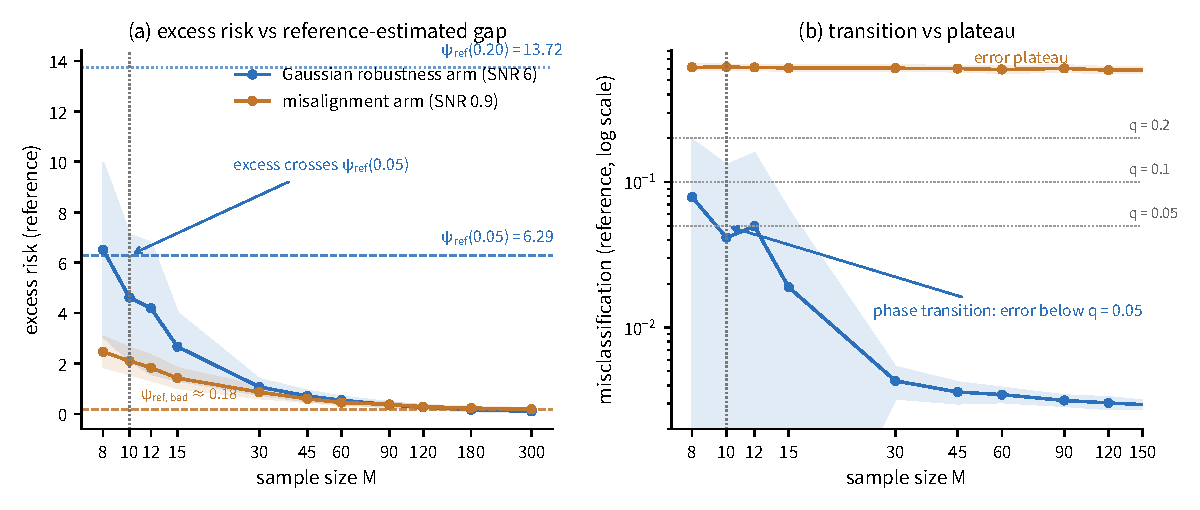
\includegraphics[width=\textwidth]{fig7_ch6_sweep.pdf}
\caption{Finite-sample sweep over sixty repetitions. Left: excess risk against sample size with the reference-estimated gap thresholds $\widehat\psi_{\rm ref}(0.05)$ and $\widehat\psi_{\rm ref}(0.20)$; the excess crosses $\widehat\psi_{\rm ref}(0.05)$ near $M=10$. These are reference-sample diagnostic thresholds, not population quantities. Right (log scale): misclassification falls below $q=0.05$ after the crossing for the aligned arm, while the negative control stays on a plateau near $0.6$. The Gaussian arm is a robustness experiment because the hard-ball assumption fails; the bounded-uniform arm is the only arm whose support condition holds analytically.}
\label{fig:sweep}
\end{figure}

The hard-ball premise deserves a design that satisfies it rather than
approximating it. The second arm, the bounded-noise theorem-compatible
arm, keeps the same geometry but replaces the Gaussian noise with
isotropic noise uniform on a ball of radius \(\rho\). The hard-ball
condition then holds almost surely by construction, and the equilateral
spacing is set to \(\Delta=6\rho\), which strictly exceeds the \(4\rho\)
the margin requires. On the reference, the empirical maximum noise norm
is exactly \(\rho\), and the nearest-center classifier at the true
centers makes no error at all. The finite-sample sweep repeats the same
fit across the same sizes and sixty repetitions: excess risk falls from
about \(0.19\) to under one hundredth, misclassification stays at zero,
and the gap implication has no violation.

The premises do not all have the same logical status. The hard-ball
support and the margin hold analytically and with probability one, while
the population alignment and the gap curve are finite-reference
diagnostics. The reference therefore gives a numerical diagnosis of the
theorem's chain, not a proof of it, and a larger reference would only
sharpen the estimate.

Three secondary robustness checks sharpen the boundary without
standalone tables. With the shape left free, the pooled fourth moment
stays non-identified as each higher moment introduces a new shape
parameter, and jointly estimating the shape does not converge in the
tested Student-\(t\) design. A median-of-means robust variant is more
stable in the specified Huber and heavy-tailed configurations, but the
non-asymptotic bound weakens as the environments approach each other. A
pre-specified grid sweep shows that underestimating \(K\) merges the
same pair while overestimating adds nested refinement with no elbow,
which supports keeping automatic selection outside the guarantees.

\subsection{The misalignment arm (negative
control)}\label{the-misalignment-arm-negative-control}

At signal-to-noise ratio nine tenths the picture changes. The true
centers misclassify close to half the reference, and the
two-versus-three-center gap shrinks to about half a unit, with the
estimated gap curve near zero. The empirical excess still declines as
the sample grows, from about \(1.48\) to under one fifth, yet
misclassification does not follow. It stays on a plateau near sixty
percent with no phase transition across the whole sweep.

That plateau is the informative result. When the population optimum is
not aligned with the true labels, adding data cannot restore them,
because the object being estimated is itself misaligned. A mechanical
count of gap violations is not meaningful here, since the gap is near
zero and its reference estimate carries finite-sample noise. We read the
arm through its one stable fact, the error plateau, and we do not report
noisy threshold crossings as counterexamples. The arm parallels the real
EEG, whose separation is of the same order and whose recovery numbers
are diagnostic, not validation.

\subsection{Summary}\label{summary-6}

The experiments establish four facts. On the Gaussian arm, where the
hard-ball support fails, the pattern stays consistent with the risk-gap
implication with no violations and a clear phase transition, an
empirical robustness result, not validation. The bounded-noise design
meets the hard-ball premise and margin analytically, while its alignment
and gap curve remain finite-reference diagnostics; it classifies with
zero error and zero violations but does not validate the chain. When the
optimum is misaligned, more data leave a stable error plateau, and the
same holds under unknown non-Gaussian shapes. The compatibility premise
stays an assumption throughout.
